\documentclass[10pt,twocolumn]{witseiepaper}

\usepackage{KJN}

\ifpdf
\pdfinfo{
/Title (ELEN4012 - Feature Based Automatic Modulation Classification)
/Author (Jacques Visser and Anthony Farquharson)
}
\fi

\begin{document}

\title{ELEN4012 - Feature Based Automatic Modulation Classification}

\author{Anthony Farquharson and Jacques Visser
\thanks{School of Electrical \& Information Engineering, University of the
Witwatersrand, Private Bag 3, 2050, Johannesburg, South Africa}
}

% TODO Rewrite abstract once the rest of the contents are figured out.
\abstract{Abstract!}

\keywords{modulation, classification, USRP, UHD}

\maketitle
\thispagestyle{empty}\pagestyle{empty}

% TODO How does one even write an introduction?
\section{INTRODUCTION}

\section{LITERATURE SURVEY}
\label{sec:literature}
According to Zhu and Nandi \cite{zhu2014automatic} there are three primary approaches to automatic modulation classification, these are: likelyhood-based, distribution-test-based and feature based. These will be discussed below.

	\subsection{Likelihood Based Classification}
	\label{subsec:likelyhood}
	Likelihood based classification is the considered the most popular method of classification, due to the accuracy of the classification when the channel is perfectly modeled \cite{zhu2014automatic}. This method requires knowledge of the channel that the signal is received from, which can be derived through evaluating every modulation hypothesis with observed signal samples \cite{zhu2014automatic}.\\[11pt]

	The main likelihood based classifier approaches are as follows \cite{zhu2014automatic}:
	\begin{itemize}
		\item \textbf{Maximum Likelihood (ML)} - This classifier requires perfect channel knowledge and all parameters are known except for the signal modulation.
		\item \textbf{Average Likelihood Ratio Test (ALRT)} - This classifier overcomes the limitation of not knowing every parameter through using accurate models for unknown parameters, making the calculation much more complex when unknown parameters are introduced.
		\item \textbf{Generalized Likelihood Ratio Test (GLRT)} - Essentially a combination of ALRT and ML classifiers, it replaces the integration of unknown parameters (ALRT) with maximization of likelihood for a possible range of unkown parameters.
		\item \textbf{Hybrid Likelihood Ratio Test (HLRT)} - The HLRT likelihood function is calculated by averaging transmitted symbols and maximizing the resulting function.
	\end{itemize}
	These classifiers are well documented by Zhu and Nandi \cite{zhu2014automatic}; Dobre, Abdi, Bar-Ness and Su \cite{dobre2007survey}. 

	\subsection{Distribution Test Based Classification}
	\label{subsec:distribution}

	\subsection{Feature Based Classification}
	\label{subsec:feature}


\section{EXISTING SOLUTIONS AND APPLICATIONS OF AMC}
	\subsection{Military}
		% jamming, listening in on communications
	\subsection{Civilian}
		% cognitive radio, effective use of bandwidth
		% aircraft monitoring

\section{SOLUTION SELECTION}

\section{DESIGN PROCESS OVERVIEW}
	\subsection{Development Methodology}
		% Engineering oriented method
		% make use of Trello
		% Add screenshots to appendix
	\subsection{Estimated Project Schedule}
		% Design, Implementation, Simulated Testing, Iteration, Practical Testing and Evaluation
		% Overview and Trello screenshots
	\subsection{Estimated Costs and Hardware Required}

\section{IMPLEMENTATION OVERVIEW}
	\subsection{Hardware}
		% USRP
		% Antenna?
		% Runs on a Linux pc, not win cos of UHD

	\subsection{Software}
		\subsubsection{Basic Software Structure}
			% fundamentally threaded
			% UHD on one thread
			% each of the feature extraction functions on their own thread
			% classifier on a final thread
		\subsubsection{Libraries and API's}

		\subsubsection{Build System}

			% Cmake because easy, also can be compiled on windows (probably UHD issue, though)

		\subsection{Feature Extraction Functions}


		\subsection{Signal Filtering}

		\subsection{Classifier}


\section{PROPOSED TESTING PROCEDURE}
	\subsection{Simulated Testing}
		% Evaluate system with generated signals
		% See how well it fares with different number of samples
		% Signal to noise ratio
	\subsection{Practical Testing}
		% correlate real world results with simulation
		% Don't make a new program, just use GNURadio companion to make signals to classify

\section{PRELIMINARY RESULTS}
	\begin{figure*}[!h]
		\centering
		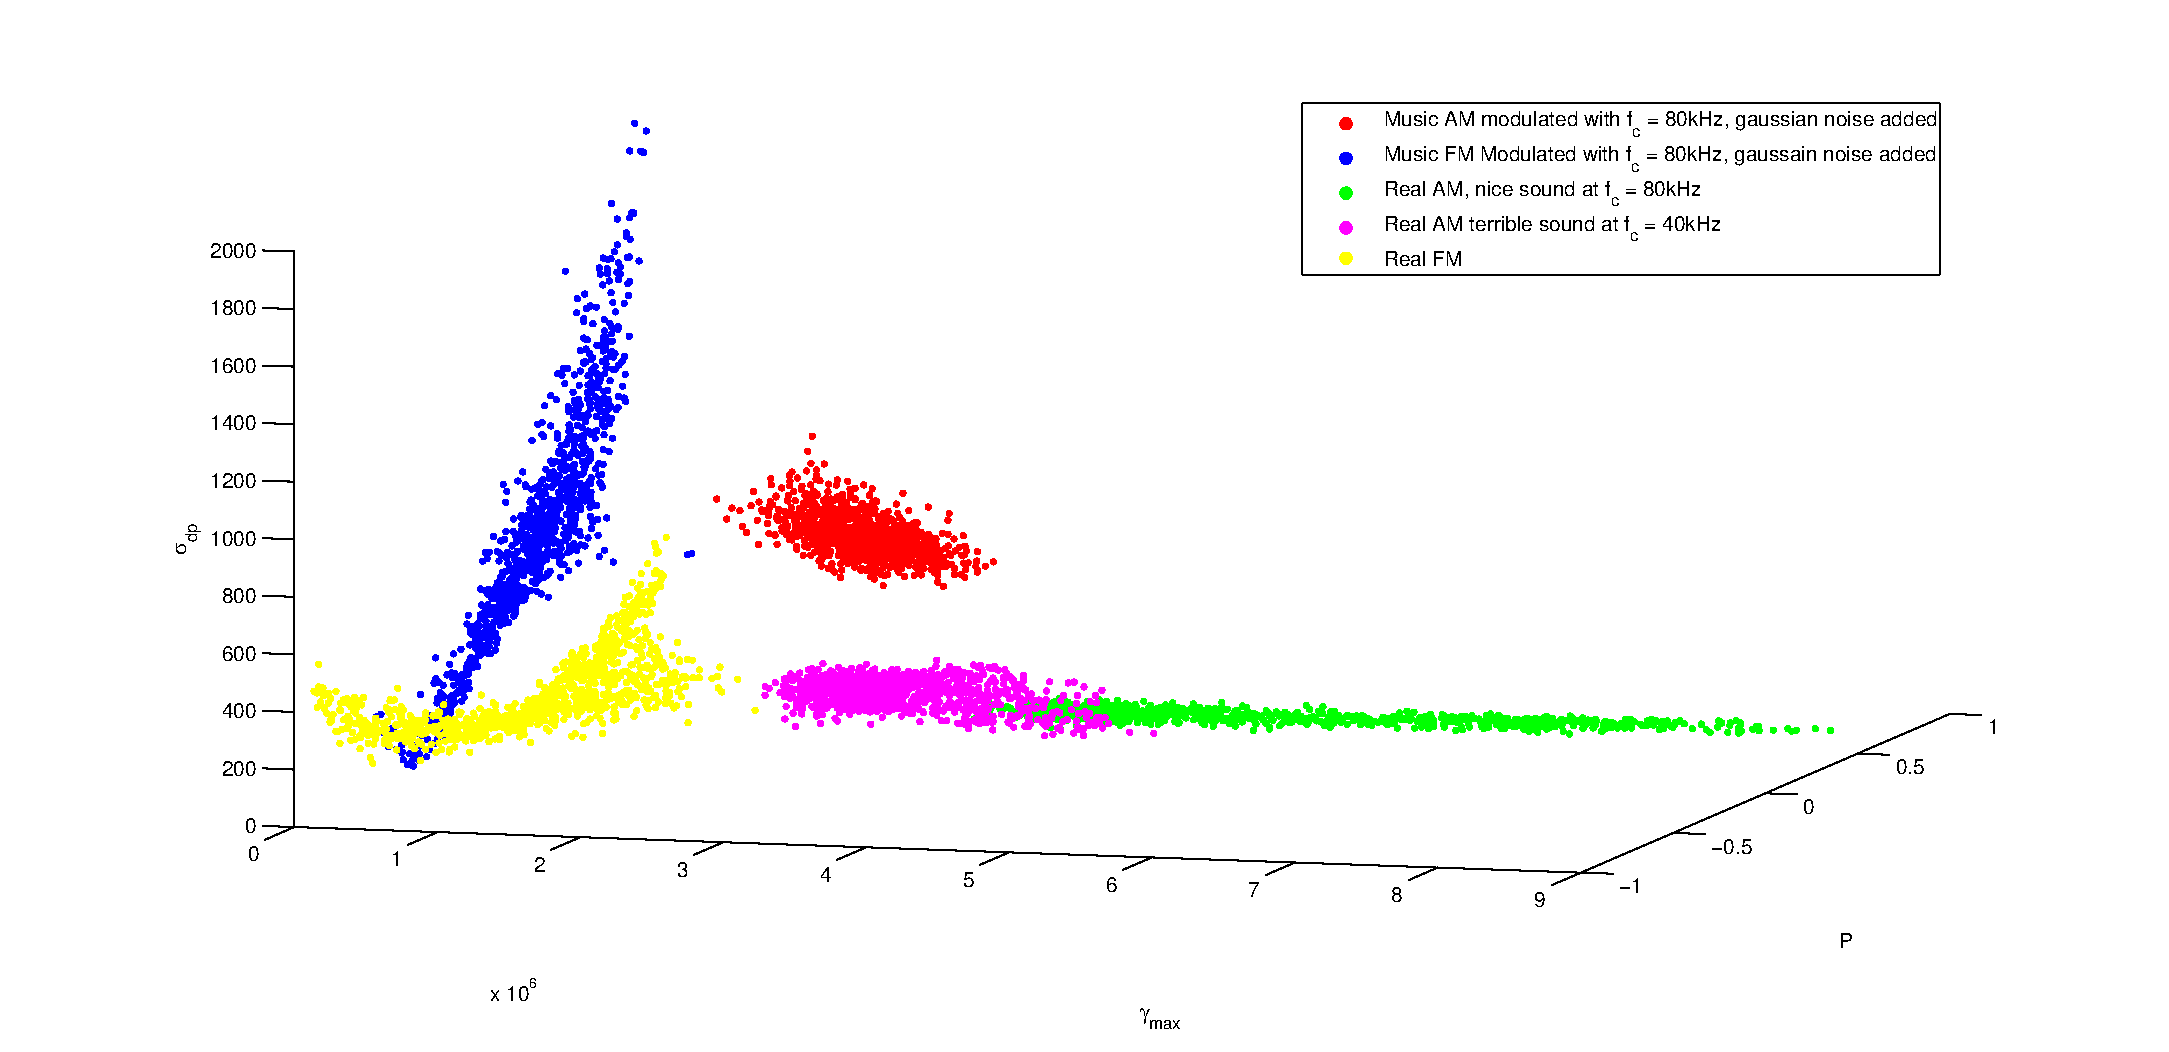
\includegraphics[width=1.1\textwidth]{plot0.eps}
		\caption{Plot of $\sigma_{dp}$ vs. $\gamma_{max}$ vs. $P$ for various AM and FM signals}
		\label{fig:plot0}
	\end{figure*}

\section{CONCLUSION AND RECOMMENDATIONS}


\bibliographystyle{witseie}
\bibliography{prelim}
\end{document}
